\documentclass{beamer}
\usetheme{Boadilla}

\usepackage[backend=biber, style=authoryear, sorting=nty]{biblatex}
\usepackage{amsmath, amssymb, amsthm, mathtools}
\usepackage{bm}
\usepackage{physics}
\usepackage{cleveref}
\usepackage{tikz}
\usetikzlibrary{positioning, backgrounds, arrows.meta}
\usepackage{pgfplots}
\usepackage{booktabs}

\pgfplotsset{compat=1.18}

\addbibresource{references.bib}

\setcounter{tocdepth}{2}


\title[Misperceived Social Norms and
Willingness to Act Against Climate Change]{Misperceived Social Norms and
Willingness to Act Against Climate Change}
\subtitle{Based on Andre, Boneva, Chopra and Peter (2024)}
\author[Theo Osterhaus]{Theo Osterhaus, 7443693}
\date[June 2026]{Climate and Human Behaviour, SuSe 2026}
\institute[WiSo]{
  Department of Economics\\
  Universität zu Köln
}

\begin{document}

\frame{\titlepage}

\begin{frame}{Outline}
    \tableofcontents
\end{frame}


\section{Motivation}

\begin{frame}{Year 2100}
    \begin{itemize}
        \item \textbf{Costs of Global Warming}\footnote{Note: 'Global warming' is a term that is used less frequently to avoid confusion with short-term or seasonal weather changes, or ozone depletion \cite{Lorenzoni2006}.}
        
        \begin{itemize}
            \item Global GDP losses of \textbf{10–25 \% by 2100} (SSP3-7.0 scenario) \cite{ipcc2023}.
            \item Pioneering study on climate economics (5–20 \% GDP loss). Stern Review (2006)
            \item \textbf{EU-Kommission (2020): }Adaptation measures \textcite{EEA2020}
        \end{itemize}

        \item Problem: Classic free riding problem: Protecting the climate comes at a personal cost
        \item How can we fight global warming?

        \begin{itemize}
            \item Institutional: Change the game/system
            \item Behavioural: Incentives, \textbf{Information}, Choice environment
        \end{itemize}
    \end{itemize}
\end{frame}

\section{Study Design}

\begin{frame}{Research Questions}
    
    \begin{enumerate}
        \item \textbf{Behavioral Determinants}:
            What factors drive individual willingness to act against climate change?
        \item \textbf{Social Norms}:
            Do misperceptions of social norms influence climate action, and if so, how?
        \item \textbf{Intervention Effect}:
            Can correcting misperceived norms increase support for climate policies?
    \end{enumerate}

\end{frame}

\begin{frame}{How to measure individuals' willingness to fight Global Warming}
    \begin{itemize}
        \item Quota-Based sampling approach of 8,000 participants \footnote{Recrutement done by \href{https://business.pureprofile.com/who-we-are/}{Pureprofile}}
        
        \begin{itemize}
            \item Representing the adult US population in terms of key sociodemographic variables, allowing us to  mitigate concerns about selection
            \item Two separate collection waves with $n=2000$ and $n=6000$
            \item Respondents could only participate in one of the two waves
        \end{itemize}
        
        \item Collect \textbf{quantitative, interpersonally comparable measure} of individuals' willingness to fight Global Warming
        \item Collect detailed Background Information of individuals' moral values, preferences and beliefs about social norms
        \item Examine if the treatment effects of Information are heterogeneous across all kinds of groups
        
    \end{itemize}
\end{frame}

\begin{frame}{Sample Characteristics}

\begin{table}[h]
    \centering
    \scriptsize 
    \begin{tabular}{lccc}
    \toprule\toprule
    Variable & Wave 1 & Wave 2 & US population (2019) \\
    \midrule
    Female                              & 51\% & 51\% & 51\% \\
    Age: 18-34                          & 30\% & 30\% & 30\% \\
    Age: 35-54                          & 32\% & 32\% & 32\% \\
    Age: 55+                            & 38\% & 38\% & 38\% \\
    Education: Bachelor's degree or above & 31\% & 31\% & 31\% \\
    Region: Northeast                   & 17\% & 17\% & 17\% \\
    Region: Midwest                     & 21\% & 21\% & 21\% \\
    Region: South                       & 38\% & 38\% & 38\% \\
    Region: West                        & 24\% & 24\% & 24\% \\
    Democrat*                           & 54\% & 53\% & 52\% \\
    Republican*                         & 46\% & 47\% & 47\% \\
    Income: Below 50k*                  & 41\% & 45\% & 37\% \\
    Income: 50k to 100k*                & 39\% & 35\% & 31\% \\
    Income: Above 100k*                 & 19\% & 20\% & 31\% \\
    \bottomrule\bottomrule
    \end{tabular}
\end{table}
    
\end{frame}

\subsection{Wave 1: Descriptive analysis (n = 2,000, March 2021)}

\begin{frame}{Wave 1: Basic descriptive facts}
\framesubtitle{Descriptive analysis (n = 2,000, March 2021)}

Wave 1 establishes the basic descriptive facts, including the widespread misperception of climate norms to measure the Pre-treatment behavior and beliefs.
    \begin{enumerate}
        \item Measuring individual willingness to fight climate change
        \item Measuring baseline behaviour and endowment of norms
        \item Measuring perceived social norms and other determinants
    \end{enumerate}
    
\end{frame}

\begin{frame}{(1) Measuring individual willingness to fight climate change}
    \begin{itemize}
        \item participants divide \$450 between themself \& \textit{atmosfair}
        \item Before respondents make their decision, the instructions provide further information on \textit{atmosfair}
    \end{itemize}

    \begin{figure}
        \centering
        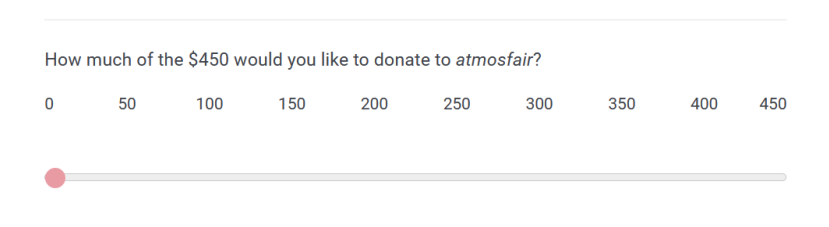
\includegraphics[width=0.75\linewidth]{Figure 7 Donation decision.png}
        \caption{Donation decision slider}
        \label{fig:placeholder}
    \end{figure}

    \begin{itemize}
        \item Results are Qunatitative \& Interpersonally comparable
        \item Probabilistic incentive scheme: Decisions of 25 randomised participants are implemented  
    \end{itemize}
    
\end{frame}

\begin{frame}{(2/3) Measuring behaviour determinats}
    \begin{itemize}
        \item Measuring baseline behaviour and endowment of norms
        
        \begin{itemize}
            \item Behaviour: 'Do you try to fight global warming?' [Yes/No] 
            \item Norms: 'Do you think that people in the United States should try to fight global warming?' [Yes/No]
        \end{itemize}
        
        \item Measuring perceived social norms
        
        \begin{itemize}
            \item Perceived behaviour: Out of 100 people we asked, how many stated that they try to fight global warming? [0-100]
            \item Perceived norms: Out of 100 people we asked, how many stated that they think that people in the United States should try to fight global warming? [0-100]
        \end{itemize}
        
    \end{itemize}
    To determine whether individual perceptions are correct, we can compare participants’ guesses with the actual shares of wave 1 respondents answering
\end{frame}

\begin{frame}{Additional Measurements}
    \begin{itemize}
        \item relationship between economic preferences and the propensity to fight global warming

        \begin{itemize}
            \item six preferences:patience, willingness to take risks, altruism, trust, positive reciprocity and negative reciprocity.
            \item preference measure is standardized to have a mean of zero and a standard deviation of one
        \end{itemize}

        \item strong reasons to hypothesize that individual willingness to fight global warming is determined by the relative importance of universal versus communal moral values

        \begin{itemize}
            \item Moral Foundations Theory (MFT),
            \item moral concerns can be partitioned into five distinct foundations: care/harm, fairness/reciprocity, in-group/loyalty, authority/respect, and purity/sanctity
        \end{itemize}
    \end{itemize}
\end{frame}

\begin{frame}{Key Problem}

\begin{alertblock}{The Misperception Gap:}
        Americans systematically underestimate how much others care.
\end{alertblock}

    
One potential concern when comparing participants’ beliefs with self-reported behaviour or norms is that participants might report an inflated tendency to behave sustainably,
e.g. due to a desire to appear good, which may result in an artificial gap between beliefs
and behaviors/norms
\end{frame}


\subsection{Wave 2}
\begin{frame}{Wave 2: Shifting perceived social norms}

\framesubtitle{Information experiment (n = 6,000, April 2021)}
    \begin{figure}
        \centering
        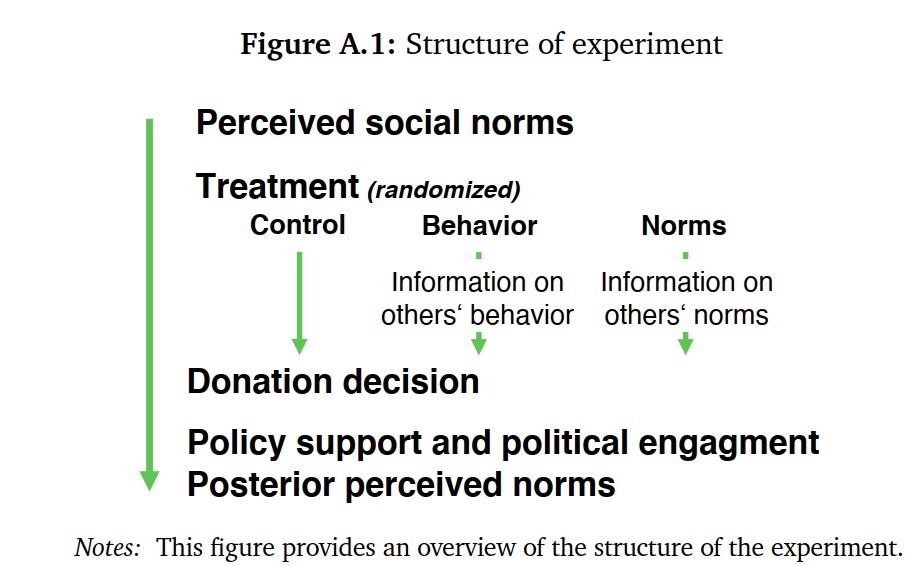
\includegraphics[width=0.75\linewidth]{Figure A.1.png}
        \label{fig:placeholder}
    \end{figure}

    If interested, have a look at the Analysis Plan of the survey of \textcite{Andre2021ClimateChange}.
    
\end{frame}



\begin{frame}{Wave 2: Information Treatment}
    \begin{itemize}
        \item Truthful information about the actual proportions of the US population who:
        \begin{itemize}
            \item (a) “try to fight global warming” (‘behavior treatment’)
            \item (b) think that “people in the US should try to fight global warming” (‘norms treatment’)
        \end{itemize}
    \end{itemize}
    \begin{figure}
        \centering
        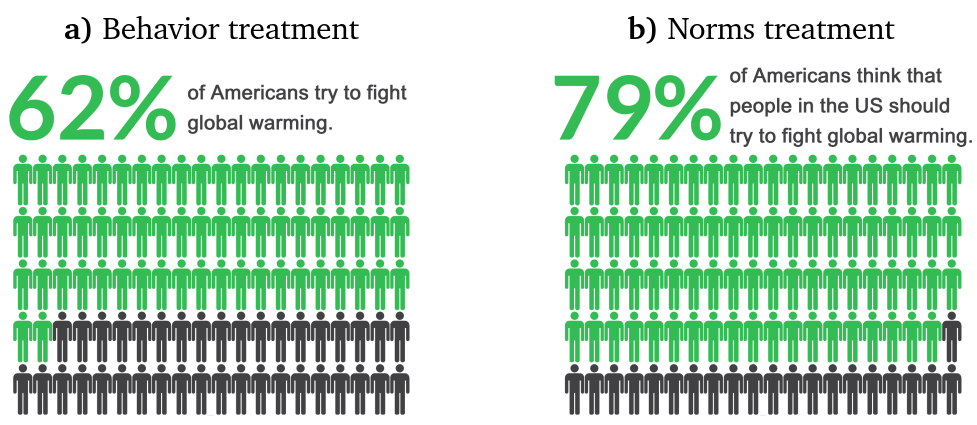
\includegraphics[width=0.7\linewidth]{Treatment.png}
        \label{fig:treatment}
    \end{figure}
    
\end{frame}

\begin{frame}{Additional measures}
    \begin{itemize}
        \item Climate change skepticism
        \item Policy support and political activism
        \item Background characteristics: We use those variables as additional control variables to increase the precision of our estimates (Statistical Power)
    \end{itemize}
    
\end{frame}

\section{Measured Outcomes and Results}
\begin{frame}{Primary Outcome: Incentivized Donation Decision}
    \begin{itemize}
        \item \textbf{Task}: Participants allocate \$450 between themselves and \textbf{\textit{atmosfair}} (climate charity).
        \item \textbf{Context}: Explained that \$450 offsets the yearly CO₂ emissions of a typical US citizen.
        \item \textbf{Procedure}: Donation amount chosen via slider (\$0–\$450).
        \item \textbf{Additional Info}: Provided details on \textit{atmosfair}’s work, expenditures, and overhead costs.
    \end{itemize}

    \vspace{0.3cm}
    \footnotesize
    \textcite{Andre2021ClimateChange} provide experimental instructions (see Section 4.3).
\end{frame}

\begin{frame}{Additional Outcome Measures}
        \begin{itemize}
            \item Baseline Behaviour and endorsement of norms
            \item Perceived Social behaviour and norms
            \item Policy support and political engagement
            \item climate change scepticism
        \end{itemize}
    
\end{frame}


\begin{frame}{Willingness to fight climate change and its determinants}
    \begin{itemize}
        \item Respondents are asked to divide \$450 between themselves and \textit{atmosfair}
        \item large heterogeneity in individual willingness to fight climate change
    \end{itemize}
    
\end{frame}

\begin{frame}{Misperceived social norms}
    
\end{frame}

\begin{frame}{Correcting misperceived social norms}
    
\end{frame}

\begin{frame}{Treatment effect heterogeneity}
    
\end{frame}

\begin{frame}{Treatment effects on policy support and political activism}
    
\end{frame}

\section{Conclusion}

\begin{frame}{Conclusion}
    \begin{itemize}
        \item Individuals' beliefs about pro-climate social norms positively predict individual donations to a climate charity
        \item We document systematic misperceptions of social norms (pluralistic ignorance)
        \item We show that correcting perceptions in an experiment causally raises individual willingness to act against climate change and individual support for climate policies
        \item The effects are strongest for individuals who are sceptical about the existence and threat of global warming
        \item Our intervention has the potential to reduce polarisation
        \item Normative beliefs positively predict pro-climate donations, comparable in strength to universal moral values and economic preferences"
    \end{itemize}
\end{frame}




\section*{Bibliography}
\begin{frame}[allowframebreaks]{Bibliography}
    \printbibliography
\end{frame}
    
\appendix
\section*{Appendix}

\begin{frame}{Formal Definition: Global Warming}
    \begin{definition}
        global warming as follows at the beginning of the survey: “ Global warming means that the world’s average temperature has considerably increased over the past 150 years and may increase more in the future.”
    \end{definition}
\end{frame}

\begin{frame}{Formal Definition: Social Norms}
    \begin{definition}
        A \textbf{social norm} is a shared expectation about appropriate behaviour in a group (Bicchieri, 2006).
    \end{definition}
    \begin{itemize}
        \item \textbf{Descriptive norm}: What people actually do.
        \item \textbf{Injunctive norm}: What people approve/disapprove of.
    \end{itemize}
\end{frame}

\begin{frame}{Nudges 2.0}
    Nudges like: defaults, social comparison, infos, labels, feedback, goal-setting\\
    Change target behaviour,\\
    Problem: modest effects, context, issue of scalability, spilover and \textbf{dampening firm behaviour} eg content of ESG label.. ;market effects eg waterbed effects and equilibria effects\\
    Use behavioral economics to INCREASE SUPPORT for efficient policies and insitutional design, self-interest, efficiency, equity, revenue recycling
    
    
    
\end{frame}



\end{document}